\chapter{Dimensionality reduction}

Supervised machine learning models in most cases require that training data or sample size \(n\) is much greater than the number of predictors or features \(p\)

\[n \gg p\]

Linear models will have high variance and overfit data as \(p\) gets closer to \(n\). If \(p = n\), ordinary least squares linear regression will perfectly fit the data, and will perform poorly an a test set.

Adding features as dimensions to a linear model will increase \(R^2\) even though the model fit quality decreases. \(R^2\) can be adjusted to number of features. It is defined as:

\[R^2_{adj} = 1 - {(n-1)RSS \over (n - p - 1)TSS}\]

WIth each added dimension, the data sparsity increases exponentially, because the volume of the data hypercube also increases exponentially. This is called the \textbf{curse of dimensionality\index{curse of dimensionality}}. Dimensionality reduction techniques help reduce the dimensionality of features while preserving as much as possible about the data conveyed.

Dimensionality reduction can be performed directly on a dataset or on a model. A number of techniques have been proposed to reduce dimensionality ranging from linear techniques to neural network based techniques.

\section{Dimensionality reduction of linear models}

Linear dimensionality reduction methods can transform a linear model to a lower number of predictors by substituting to another smaller set of predictors.

Let the following be a linear model

\[Y = \beta_0 + \sum_{i=1}^p\beta_iX_i\]

Where \(Y\) and \(X_i\) are a vector of size \(n\), where \(n\) is the sample size. We can define a linear transformation to a lower dimension \(M\), as

\[Z_m = \sum_{j=1}^p \phi_{jm}X_j\]

where \(M<p\) and \(m = 1,...,M\) and \(\phi_{jm}\) are the parameters for dimensionality reduction. We can rewrite our model with the new parameters \(Z_m\) as:

\[Y = \theta_0 + \sum_{m=1}^M\theta_mZ_m\]

We can fit this model with less parameter: \(M + 1\), compared to \(p + 1\), where \(M < p\). We can fit the model with ordinary least squares in the same way we would fit the original model. It's called dimensionality reduction, because we reduced the number of model parameters.

The relationship between the model parameters are:

\[\beta_j = \sum_{m = 1}^M\theta_m \phi_{jm}\]

So far we omitted the task on choosing the \(\phi_{jm}\) parameters. Depending on how we choose them, OLS on the reduced model might provide a better fit. Linear dimensionality techniques can be used to reduce both the data directly as well as the linear models.

\section{Principal Component Analysis}

\textbf{Principal Component Analysis\index{Principal Component Analysis}} (PCA) is a form of \textbf{unsupervised learning\index{unsupervised learning}}, which means no labeled training dataset is needed. PCA can be used to reduce the dimension of an \(n \times p\) matrix.

The PCA method remaps the basis vectors of the dataset (in Figure 8.1 the basis vectors are unit vectors on the axis \(X_1\) and \(X_2\) respectively). The first principal component we choose in PCA is the one where the variance of the data is maximum (in Figure 8.1 the diagonal continuous line). Projecting the observations to the line of the first principal component results in the largest variance of the projected data, compared to any other line. In other words, the first principal component is the line closest to the data.


\begin{figure}[htbp]
    \begin{center}
        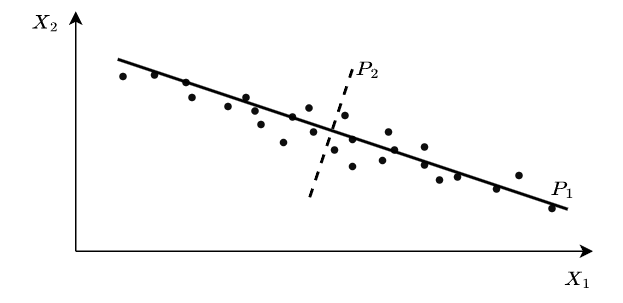
\includegraphics[width=250pt]{../img/08-principal-component.png}
        \caption{Figure 8.1:  Principal components of a two dimensional dataset}
    \end{center}
\end{figure}


Since in the example there is high correlation between \(X_1\) and \(X_2\), the first principal component captures this relationship. The second component is chosen to capture the remaining maximum variance, in this case the remaining variance. Principal components are uncorrelated, so they are perpendicular to one another.

When we have \(p\) features, we can choose in similar manner up to \(p\) principal components. Since we maximize capturing variance with each component we can limit the number of components to \(M\), where \(M < p\), resulting in dimensionality reduction, while still minimizing data loss.

To compute the principal components we use spectral decomposition. For a full treatment on linear algebra, eigenvalues, eigenvectors and matrix decomposition, see Appendix II. For a data matrix \(X\) (where each row is an observation and columns are the features \(X_1, ..., X_n\)) the algorithm for PCA is as follows:

\begin{enumerate}
    \item \textbf{Center the Data\index{Center the Data}}: Before PCA is applied, the data is usually centered. This means subtracting the mean of each feature from the data so that the mean of the centered data is zero.
    \item \textbf{Compute the Covariance Matrix\index{Compute the Covariance Matrix}}: For the centered data matrix \(X\), compute the covariance matrix \(\Sigma\) given by: \[\Sigma = \frac{1}{n-1} X^T X\] Where \(n\) is the number of observations.
    \item \textbf{Spectral decomposition of the Covariance Matrix\index{Spectral decomposition of the Covariance Matrix}}: Compute the eigenvectors and eigenvalues of the covariance matrix \(\Omega\). Since \(\Omega\) is the form of \(X^T X\) scaled by a constant, means it's a symmetric matrix, which in turn means that its eigenvectors are orthogonal, and can be decomposed using spectral decomposition. Let \(V\) be the matrix whose columns are the eigenvectors of \(\Sigma\) and \(\lambda\) be the corresponding eigenvalues. Using spectral decomposition will have the form of:
\[\Omega = V \Sigma V^T \]
    \item \textbf{Order the Eigenvectors\index{Order the Eigenvectors}}: Sort the eigenvectors in \(V \) in descending order based on the magnitude of their corresponding eigenvalues in \(\Sigma\). The reason for this is that the largest eigenvalue corresponds to the direction of the greatest variance in the data, the second largest to the second most direction of variance, and so on.
    \item \textbf{Principal Components\index{Principal Components}}: The sorted eigenvectors are the principal components. They provide an orthogonal basis for the data space, with each component capturing a descending amount of the total variance in the data. These are the first \(k\) columns of \(V\), noted with \(V_k\).
    \item \textbf{Projection\index{Projection}}: The original data \(X\) can be projected onto these top \(k\) principal components (or right singular vectors) using:
\end{enumerate}

\[X_k=XV_k\]

The principal components essentially provide a new coordinate system for the data where the axes are aligned with the directions of maximum variance (as determined by the eigenvectors of the covariance matrix). By ordering these axes by the amount of variance they capture (as determined by the eigenvalues), we can efficiently reduce the dimensionality of the data, if desired, by only considering the most significant axes.

\section{Autoencoders}


